\documentclass[11pt, oneside]{article}   	% use "amsart" instead of "article" for AMSLaTeX format
\usepackage{geometry}                		% See geometry.pdf to learn the layout options. There are lots.
\geometry{letterpaper}                   		% ... or a4paper or a5paper or ... 
%\geometry{landscape}                		% Activate for for rotated page geometry
%\usepackage[parfill]{parskip}    		% Activate to begin paragraphs with an empty line rather than an indent
\usepackage{graphicx}				% Use pdf, png, jpg, or eps� with pdflatex; use eps in DVI mode
								% TeX will automatically convert eps --> pdf in pdflatex		
\usepackage{amssymb}
\graphicspath{{/Users/telliott_admin/Dropbox/Tex/png/}}

\title{Infinite Series}
%\author{The Author}
\date{}							% Activate to display a given date or no date

\begin{document}
\maketitle
%\section{}
%\subsection{}
\large
\noindent My favorite infinite series is this one:
\[ 1 + \frac{1}{2} + \frac{1}{4} + \frac{1}{8} + \cdots \]
It is called the geometric series because each term is the product of the previous one times a constant ratio $r=1/2$.  We can also write this compactly as as
\[ \sum_{k=0}^\infty \frac{1}{2^k} \]
One way to solve this, to find the value of the sum, is to suppose that it has a sum S (but beware)
\[ S = 1 + \frac{1}{2} + \frac{1}{4} + \frac{1}{8} + \cdots \]
Looks all right.  Then do some algebra
\[ \frac{S}{2} = \frac{1}{2} + \frac{1}{4} + \frac{1}{8} + \frac{1}{16} + \cdots \]
\[ S - \frac{S}{2} = 1 + \frac{1}{2} + \frac{1}{4} + \frac{1}{8} + \cdots \ \ \ - \frac{1}{2} + \frac{1}{4} + \frac{1}{8} + \frac{1}{16} + \cdots = 1 \]
It turns that out the answer is correct, even the method has some issues.  That is, provided that \emph{the sum is not infinite}, this works.  One way to see that it cannot work in general is this counterexample
\[ S = 1 + 2 + 4 + 8 + \cdots \]
\[ 2S = 2 + 4 + 8 + 16 + \cdots \]
\[ S - 2S = 1 \]
\[ S = -1 \ \ ??? \]
Going back to the first series, and leaving out the first term, there is a beautiful visual proof that 
\[ \frac{1}{2} + \frac{1}{4} + \frac{1}{8} + \cdots = 1 \]
\begin{center}
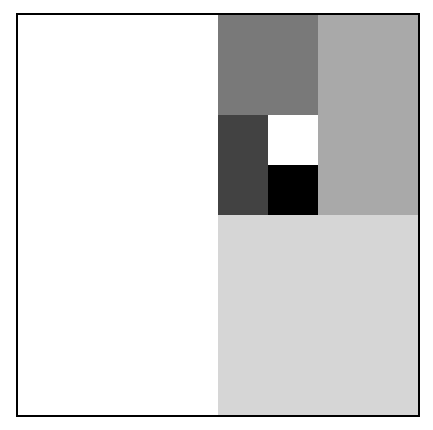
\includegraphics [scale=0.5] {series1.png}
\end{center}
We have a square of area 1, in the first step we color ($1/2$) the square white, then we take half of what remains ($1/4$) and color it light gray, then take half of what remains after that($1/8$) and color it medium gray, and so on.  Since at each step we take half of what remains, and since this process can continue forever, we must end up with $1$.  The sum including the first term is then equal to $2$.

There are many other infinite series.  We could mention three that are most important
\[ e^x = 1 + x + \frac{x^2}{2!} + \ldots  \]
\[ sin \ x = x - \frac{x^3}{3!} + \frac{x^5}{5!}  - \frac{x^7}{7!} + \ldots \]
\[ cos \ x =  1  - \frac{x^2}{2!} + \frac{x^4}{4!}  - \frac{x^6}{6!} + \ldots \]

These can be used to demonstrate various properties of the functions, for example that $\frac{d}{dx} e^x = e^x$, and similarly that $\frac{d}{dx} sin\ x = cos\ x$.  I say "demonstrate" because, at least for the trigonometric functions, the "proof" is circular.  One must use the calculus of sine and cosine to derive the series (AFAIK).

Finally, it is worth dealing with how one would prove this result about the first series algebraically.  Let 
\[ S = 1 + r + r^2 + r^3 + \cdots \]
\[ Sr = r + r^2 + r^3 + \cdots \]
\[ S - Sr = S(1-r) = 1 \]
\[ S = \frac{1}{1-r} \]
The idea is that this is only true if this series is \emph{convergent}.  How do we show that?  We think about taking the series out to some point $n=k$.  Then we multiply by $1-r$ and we have
\[ (1-r)(1 + r + r^2 + r^3 + \cdots + r^k ) = \]
We get two series, one on top of the other
\[ 1 + r + r^2 + r^3 + \cdots + r^k  \]
\[ - r - r^2 - r^3 + \cdots - r^k - r^{k+1} \]
This is what's called a "collapsing sum."  The sum of the two series is
\[ 1 - r^{k+1} \]
As $k$ gets very large, the term $r^{k+1}$ gets small, \emph{as long as} $-1 < r < 1$.  So the series converges and
\[ (1-r)(1 + r + r^2 + r^3 + \cdots ) = 1 \]
\[ S = \frac{1}{1-r} \]
But only if $r<1$.  This is called the "radius of convergence."  In the example that gave problems above, r = 2.
Here is another one
\[ S = \frac{1}{2} + \frac{1}{3} + \frac{1}{4} + \frac{1}{5} + \frac{1}{6} + \frac{1}{7}+ \frac{1}{8} + \cdots  \]
\[ S = \frac{1}{2} + (\frac{1}{3} + \frac{1}{4}) + (\frac{1}{5} + \frac{1}{6} + \frac{1}{7}+ \frac{1}{8})  + \cdots  \]
The terms of the series can be grouped so that each group has a sum $> 1/2$.
\[ (\frac{1}{3} + \frac{1}{4}) > \frac{1}{2} \]
\[ (\frac{1}{5} + \frac{1}{6} + \frac{1}{7}+ \frac{1}{8}) > \frac{1}{2} \]
So the sum of the series is larger than this one
\[ S = \frac{1}{2} + \frac{1}{2} + \frac{1}{2} + \cdots  \]
which is clearly divergent.

A last example is
\[ 1 + \frac{1}{3}  + \frac{1}{6}  + \frac{1}{10}  + \frac{1}{15} + \cdots \]
The denominators are the "triangular" numbers from Pascal's triangle.
Factor out 2
\[ 2\ [\frac{1}{2} + \frac{1}{6}  + \frac{1}{12}  + \frac{1}{20}  + \frac{1}{30} + \cdots \ ]\]
\[ 2\ [(1-\frac{1}{2}) + (\frac{1}{2}-\frac{1}{3})  + (\frac{1}{3}-\frac{1}{4})  + (\frac{1}{4} - \frac{1}{5})  + (\frac{1}{5}-\frac{1}{6}) + \cdots \ ] \]
All the terms cancel except for
\[ 2\ [ 1] = 2 \]

\end{document}  